\documentclass[12pt]{article}
\usepackage[top=1in,left=1in, right = 1in, footskip=1in]{geometry}

\usepackage{graphicx}
\usepackage{xspace}
%\usepackage{adjustbox}

\newcommand{\comment}{\showcomment}
%% \newcommand{\comment}{\nocomment}

\newcommand{\showcomment}[3]{\textcolor{#1}{\textbf{[#2: }\textsl{#3}\textbf{]}}}
\newcommand{\nocomment}[3]{}

\newcommand{\jd}[1]{\comment{cyan}{JD}{#1}}
\newcommand{\swp}[1]{\comment{magenta}{SWP}{#1}}
\newcommand{\bmb}[1]{\comment{blue}{BMB}{#1}}

\newcommand{\eref}[1]{Eq.~\ref{eq:#1}}
\newcommand{\fref}[1]{Fig.~\ref{fig:#1}}
\newcommand{\Fref}[1]{Fig.~\ref{fig:#1}}
\newcommand{\sref}[1]{Sec.~\ref{#1}}
\newcommand{\frange}[2]{Fig.~\ref{fig:#1}--\ref{fig:#2}}
\newcommand{\tref}[1]{Table~\ref{tab:#1}}
\newcommand{\tlab}[1]{\label{tab:#1}}
\newcommand{\seminar}{SE\mbox{$^m$}I\mbox{$^n$}R}

\usepackage{amsthm}
\usepackage{amsmath}
\usepackage{amssymb}
\usepackage{amsfonts}

\usepackage{lineno}
\linenumbers

\usepackage[pdfencoding=auto, psdextra]{hyperref}

\usepackage{natbib}
\bibliographystyle{chicago}
\date{\today}

\usepackage{xspace}
\newcommand*{\ie}{i.e.\@\xspace}

\usepackage{color}

\newcommand{\Rx}[1]{\ensuremath{{\mathcal R}_{#1}}\xspace} 
\newcommand{\Ro}{\Rx{0}}
\newcommand{\Rc}{\Rx{c}}
\newcommand{\RR}{\ensuremath{{\mathcal R}}\xspace}
\newcommand{\Rhat}{\ensuremath{{\hat\RR}}}
\newcommand{\Rnaive}{\ensuremath{{\mathcal R}_{\textrm{\tiny naive}}}\xspace}
\newcommand{\tsub}[2]{#1_{{\textrm{\tiny #2}}}}
\newcommand{\dd}[1]{\ensuremath{\, \mathrm{d}#1}}
\newcommand{\dtau}{\dd{\tau}}
\newcommand{\dx}{\dd{x}}
\newcommand{\dsigma}{\dd{\sigma}}
\begin{document}

\begin{flushleft}{
	\Large
	\textbf\newline{
		Unraveling the paradox between generation and serial intervals: applications to the COVID-19 pandemic
	}
}
\end{flushleft}

\section*{Abstract}

Generation and serial intervals are under-appreciated --- often treated as auxiliary variables for estimating the reproduction number \RR --- yet important quantities in understanding the outset of an outbreak.
We argue that a part of the confusion can be attributed to an apparent paradox.
\bmb{need to define the paradox here, e.g.: ``although they cannot be used interchangeably in analyzing the behaviour of an epidemic, they give rise to nearly identical relationships between the epidemic growth rate $r$ and \RR''}
As the generation-interval distribution describes the renewal process of infection, it provides a link between the epidemic growth rate $r$ and the reproduction number \RR;
likewise, the serial-interval distribution should describe the renewal process of symptomatic infection and therefore, should provide the same link between the epidemic growth rate $r$ and the reproduction number \RR.
%However, the current theory does not explain how two different distributions can give the same link between $r$ and $\mathcal R$ link.
We provide an answer to the paradox by showing that if serial intervals are defined as \emph{forward-looking} intervals during the exponential phase, then the correct link between $r$ and \RR emerges.
We also provide a heuristic way of addressing potential biases that can arise from not accounting for changes in these references.
Our study reveals gaps in the current understanding of serial intervals and provides rationale for reassessing serial intervals of COVID-19.

\pagebreak

\section{Introduction}

The reproduction number \RR is one of the most important characteristics of an emerging epidemic such as novel coronavirus disease (COVID-19) \citep{majumder2020early} \bmb{avoid starting a paper by saying ``X has been studied a lot''; instead, say it's important or interesting}
The reproduction number is defined as the average number of secondary cases caused by a primary case;
the corresponding reproduction number in a fully susceptible population --- referred to as the basic reproduction number \Ro --- allows us to predict the extent to which a disease will spread in the population and the amount of intervention to prevent an outbreak \citep{anderson1991infectious}.
Since reproduction number cannot be measured directly, particularly during the outset of an outbreak, it is often estimated from the observed exponential growth rate using generation- and serial-interval distributions (e.g., \cite{du2020serial, jung2020real, li2020early, zhao2020preliminary}).

The generation interval is defined as the time between when an individual (infector) is infected and when an individual infects another person (infectee);
the generation-interval distribution determines the relationship between the exponential growth rate $r$ and the reproduction number \RR \citep{wallinga2007generation}.
Similarly, the serial interval is defined as the time between when an infector and an infectee become \emph{symptomatic} \citep{svensson2007note}.
While serial intervals are similar to generation intervals, previous studies have noted that, in many contexts, serial intervals are expected to have larger variances than generation intervals but have the same mean \citep{svensson2007note,klinkenberg2011correlation,te2013estimating,champredon2018equivalence};
some studies further suggested that using serial intervals can give different estimates of \RR \citep{britton2019estimation}.
Even these distributions were clearly distinguished over a decade ago \citep{svensson2007note}, 
the need for a better conceptual and theoretical framework for understanding their differences is becoming clearer as the COVID-19 pandemic unfolds:
Researchers continue to rely on both generation and serial intervals to estimate \RR for COVID-19 without making a clear distinction.

One important source of confusion comes down to an apparent paradox.
When the epidemic is growing exponentially, the spread of infection can be characterized as a ``renewal process'' based on previous incidence of infection, the associated generation-interval distribution, and the average infectiousness of an infected individual.
This renewal formulation allows us to link the exponential growth rate of an epidemic $r$ with its reproduction number \RR \citep{wallinga2007generation}.
Likewise, we should be able to describe the renewal process of symptomatic cases using the serial-interval distribution.
Therefore, both generation- and serial-interval distributions should give us identical estimates of  \RR based the observed epidemic growth rate $r$.
In contexts where the distributions are expected to be different, current theory has no explanation for how they might link $r$ to \Rx\ in the same way.

Here, we provide an answer to this paradox, by showing that the relevant interval for the renewal framework is what is called the ``forward'' interval, and that the forward serial (but not generation) interval is affected by the rate of growth $r$ during the exponential-growth phase.
We develop a new framework for understanding serial intervals and show that the initial forward serial-interval distribution gives the correct value of \RR.
%\jd{Come back to this. Not just over time, right?} \swp{What do you mean? Everything is about time here... you haven't read the results section so maybe that's why?}
However, using inaccurately defined serial intervals or failing to account for changes in the observed serial-interval distributions over the course of an epidemic can bias the estimate of \RR.
We apply our framework to serial intervals of COVID-19 and lay out several principles to consider in using information about serial intervals and other epidemiological time delays in the analysis of the ongoing pandemic.

\section{Methods}

\subsection{Backward and forward delay distributions}

We first begin by describing a general framework for characterizing a distribution of time delays between two epidemiological events;
these events can be defined either within an infected individual (e.g., infection and symptom onset of an individual, the incubation period) or between infected individuals (e.g., symptom onsets of an infector and an infectee, the serial interval).
We can further divide these events into \emph{primary} and \emph{secondary} events.
When we measure an epidemiological time delay within an infected individual (e.g., the incubation period), the primary event is the event that always or usually occurs before the secondary event ---
most epidemiological events that can be observed within an individual have clear direction (e.g., infection and onset of symptoms) but some may not (e.g., onset of infectiousness and onset of symptoms).
% \jd{Rethink, or else rethink ``any'' above: the ``hidden'' time (my term) is the time between onset of infectiousness and onset of symptoms; it is within, but can be positive or negative. I'm not saying we should use it here\ldots}
When we measure an epidemiological time delay between infected individuals (e.g., the serial interval), 
the primary and secondary events are defined in terms of the direction of transmission:
The primary event refers to the event that occurs within an infector and does not necessarily occur before the secondary event.

We model time delays between a primary and a secondary event from a cohort perspective.
A primary cohort consists of \emph{all} individuals whose primary event occurred at a given time; 
a secondary cohort is defined similarly based on the secondary events.
For example, when we are measuring serial intervals, a primary cohort $\pi$ consists of all infectors who became symptomatic at time $\pi$.
Then, for each primary cohort $\pi$, we can define the expected time distribution between primary and secondary events.
We refer to this distribution as the forward delay distribution and denote it as $f_\pi(\tau)$.

Likewise, we define the backward delay distribution $b_\delta(\tau)$ for a secondary cohort $\delta$:
The backward delay distribution describes the time delays between a primary and secondary host given that the secondary event occurred at time $\delta$.
Since both forward and backward perspectives provide valid ways of measuring time delays, we can express the total density of primary and secondary events occurring at time $\pi$ and $\delta$, respectively, using both forward and backward delay distributions:
\begin{equation}
P(\pi) f_\pi(\delta-\pi) = D(\delta) b_\delta(\delta-\pi),
\end{equation}
where $P$ and $D$ represent the sizes of primary and secondary cohorts, respectively.
Substituting $\tau = \delta - \pi$, it follows that:
\begin{equation}
b_\delta(\tau) = \frac{P(\delta-\tau) f_{\delta-\tau}(\tau)}{D(\delta)}
\end{equation}
Therefore, the backward delay distribution depends on the changes in primary cohort size $P$ (therefore incidence of infection) as well as changes in the forward delay distribution.
These ideas apply to all epidemiological delay distributions and generalize the work by \citep{champredon2015intrinsic} who compared forward and backward generation-interval distributions to describe the realized generation intervals from the perspective of an infector and an infectee, respectively.
\bmb{need to work \textbf{really hard} to clarify the mechanisms driving various differences [backward vs forward, dependence on current $S$/epidemic phase, etc.]; which are caused by changes in cohort size over time (Euler-Lotka-type effects), which are caused by censoring/conditionality of observations, etc. ?}

\subsection{Realized serial interval distributions}

The serial interval is defined as the time between when an infector becomes symptomatic and when and infectee becomes symptomatic.
Serial intervals $\tau$ have been typically written in the form:
\begin{equation}
\tau = - x_0 + \sigma + x_1
\end{equation}
where $x_0$ and $x_1$ represent the realized time from infection to symptom onset of an infector and an infectee, respectively, and $\sigma$ represents the realized generation interval.
Previous studies have often assumed that $x_0$ and $x_1$ follow the same distributions and concluded that the serial and generation intervals have the same mean \citep{svensson2007note,klinkenberg2011correlation,champredon2018equivalence, britton2019estimation}.
% \jd{I would drop the last clause. I still argue that this is true for intrinsic SIs, and we don't want to get into that here. You can just keep rolling forward at this point.}

\begin{figure}[!th]
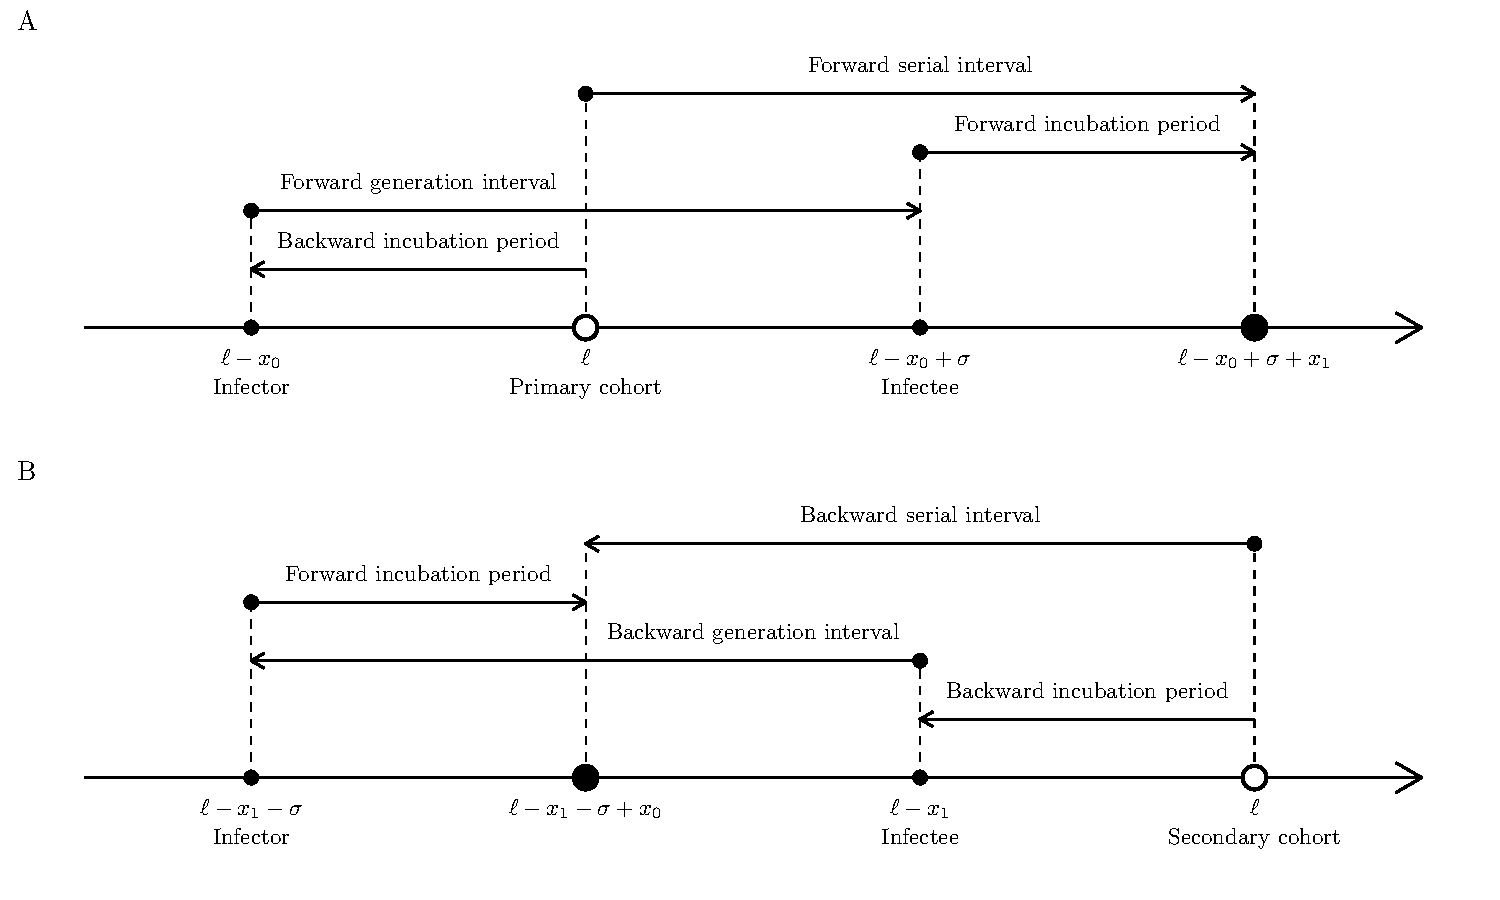
\includegraphics[width=\textwidth]{serial_guide.pdf}
\caption{
\textbf{Illustration of forward and backward serial intervals.}
(A) The forward serial interval for a primary cohort $\pi$ (i.e., an infector who became symptomatic at time $\pi$).
In this case, $x_0$ represents the backward incubation period of the infector;
$\sigma$ represents the forward generation interval;
and $x_1$ represents the forward incubation period of the infectee.
(B) The backward serial interval for a secondary cohort $\delta$ (i.e., an infectee who became symptomatic at time $\delta$).
In this case, $x_0$ represents the forward incubation period of the infector;
$\sigma$ represents the backward generation interval;
and $x_1$ represents the backward incubation period of the infectee.
}
\label{fig:diagram}
\end{figure}

The cohort-based framework allows us to understand the distribution of serial intervals we expect to observe when incidence is changing.
Given that an infector became symptomatic at time $\pi$, we first go backward in time by asking when the infector was infected, and then go forward in time by asking first when the infectee was infected and then when the infectee became symptomatic;
this defines the forward serial interval.
In \fref{diagram}A, we see that $x_0$ represents the backward incubation period of the infector who became symptomatic at time $\pi$;
$\sigma$ represents the forward generation interval of the infector who came infected at time $\pi - x_0$;
and $x_1$ represents the forward incubation period for the infectees who became infected at time $\pi - x_0 + \sigma$.

Likewise, we can define the backward serial interval distribution for a secondary cohort $\delta$ (\fref{diagram}B).
Given that an infectee became symptomatic at time $\delta$, we have to first go backward in time by asking when the infectee became infected and when the infector became infected; 
then, we have to go forward in time by asking when the infector became symptomatic.
In this case, $x_1$ represents the backward incubation period of the infectee who became symptomatic at time $\delta$;
$\sigma$ represents the backward generation interval of the infectee who became infected at time $\delta-x_1$;
and $x_0$ represents the forward incubation period of the infector who became infected at time $\delta-x_1-\sigma$.
This conceptual framework clearly demonstrates that the distributions of $x_0$, $\delta$, and $x_1$ (and therefore the distributions of serial intervals) depend on the perspective \bmb{better/more consistent word than ``perspective''?} as well as time and cannot be treated statically.
\bmb{please explain/clarify why the backward incubation period is not the same is as the forward}

In order to define forward and backward serial interval distributions, we begin by writing the total number of serial intervals \bmb{explain more please \ldots} between time $\pi$ (when the infector developed symptoms) and $\delta$ (when the infectee developed symptoms), which can be expressed as an integral over all of the possibilities for the infection times of the infector $\alpha_1$ and the infectee $\alpha_2$:
\begin{equation}
T(\pi,\delta) = \int_{-\infty}^{\pi} \int_{\alpha_1}^{\delta} \Rc (\alpha_1) i(\alpha_1) h_{\alpha_1}(\pi-\alpha_1, \alpha_2 - \alpha_1) k_{\alpha_2}(\delta - \alpha_2) \, \mathrm{d}\alpha_2\,\mathrm{d}\alpha_1,
\end{equation}
where $\Rc(\alpha_1)$ is the case reproduction number (i.e., the average number of secondary cases caused by a primary case infected at time $\alpha_1$, \cite{fraser2007estimating}) \bmb{is \Rc the same as ``forward \R measured at a particular time''?}, $i(\alpha_1)$ is incidence, $h_{\alpha_1}(\pi-\alpha_1, \alpha_2 - \alpha_1)$ is the joint probability distribution describing the forward incubation period $\pi-\alpha_1$ and forward generation interval $\alpha_2 - \alpha_1$ of an individual infected at time $\alpha_1$ (in this case, the infector), and $k_{\alpha_2}(\delta-\alpha_2)$ describes the marginal probability distribution of $h_{\alpha_2}$ describing the forward incubation period $\delta-\alpha_2$ of an individual infected at time $\alpha_2$ (in this case, the infectee). 
Then, the forward serial-interval distribution is proportional to $T(\pi, \pi+\tau)$. Substituting $x=\pi-\alpha_1$ and $\sigma=\alpha_2-\alpha_1$, we have:
\begin{equation}
f_\pi(\tau) \propto \int_{0}^{\infty} \int_{0}^{\max(0,x+\tau)} \Rc (\pi-x) i(\pi-x) h_{\pi-x}(x, \sigma) k_{\pi-x+\sigma}(x-\sigma+\tau) \dsigma \dx
\end{equation}
Likewise, the backward serial-interval distribution is proportional to $T(\delta-\tau, \delta)$. 
This time, we substitute $x=\delta-\alpha_2$ and $\sigma=\alpha_2-\alpha_1$ to get:
\begin{equation}
b_\delta(\tau) \propto \int_{0}^{\infty} \int_{\max(0, \tau-x)}^{\infty} \Rc (\delta-x-\sigma) i(\delta-x-\sigma) h_{\delta-x-\sigma}(x+\sigma-\tau, \sigma) k_{\delta-x}(x) \dsigma \dx.
\end{equation}

\subsection{Epidemic model}

We validate \bmb{??} the theory by applying it to a specific example of an epidemic model. 
We model disease spread with a renewal-equation model \citep{heesterbeek1996concept, diekmann2000mathematical, roberts2004modelling, aldis2005integral, roberts2007model, champredon2018equivalence}.
Ignoring births and deaths, changes in the proportion of susceptible individuals $S(t)$ and incidence of infection $i(t)$ can be written as:
\begin{equation}
\begin{aligned}
\frac{\mathrm{d}S}{\mathrm{d}t} &= - i(t)\\
i(t) &= \Ro S(t) \int_0^\infty i(t-\tau) g(\tau) \dtau,
\end{aligned}
\label{eq:renewal}
\end{equation}
where \Ro is the basic reproduction number, and $g(\tau)$ is the intrinsic generation-interval distribution (i.e., the forward generation-interval distribution of a primary case in a fully susceptible population; \cite{champredon2015intrinsic}).
Then, the forward generation-interval for a primary cohort $\pi$ follows \citep{champredon2015intrinsic}:
\begin{equation}
g_\pi (\tau) \propto g(\tau) S(\pi + \tau),
\end{equation}
which allows us to separate the joint probability distribution $h_\pi$ of the forward incubation period and the forward generation-interval distribution as a product of the proportion of susceptible individuals $S$ and the joint probability distribution $h$ of the forward incubation period and the intrinsic generation intervals:
\begin{equation}
h_\pi (x, \tau) \propto h(x, \tau) S(\pi + \tau).
\end{equation}
We further assume that the forward incubation period distributions does not vary across cohorts over the course of an epidemic, as they represent the natural history of a disease, and use $k$ without subscript instead. 
Then, we have:
\begin{equation}
\begin{aligned}
k(x) &= \int_0^\infty h(x, \tau) \dtau\\
g(\tau) &= \int_0^\infty h(x, \tau) \dx
\end{aligned}
\end{equation}
Finally, the case reproduction for this model is defined as follows:
\begin{equation}
\Rc(t) = \Ro \int_0^\infty g(\tau) S(t+\tau) \dtau.
\end{equation}

\subsection{Linking $r$ and \RR}

During the initial phase of an epidemic, the proportion susceptible remains approximately constant ($S(t) \approx S(0)$) and incidence of infection grows exponentially: $i(t)=i_0\exp(rt)$.
Then, we can use the Euler-Lotka equation to estimate the reproduction number from the exponential growth rate $r$ \bmb{ref??}:
\begin{equation}
\frac{1}{\RR} = \int_0^\infty \exp(-r\tau) g(\tau) \dtau.
\end{equation}
Analogous to forward generation-interval distributions, 
forward serial-interval distributions describe the renewal process of symptomatic cases.
Therefore, we expect the forward serial-interval distribution during the exponential growth phase --- which we refer to as the \emph{initial} forward serial-interval distribution $f_0$ --- to provide the identical $r$--\RR link as the intrinsic generation-interval distribution:
\begin{equation}
\frac{1}{\RR} = \int_{-\infty}^\infty \exp(-r\tau) f_{0}(\tau) \mathrm{d} \tau,
\end{equation}
where the initial forward serial-interval distribution is defined as:
\begin{equation}
f_{0}(\tau) \propto \int_{0}^{\infty} \int_{0}^{\max(0,x+\tau)} \exp(-rx) h(x, \sigma) k(x-\sigma+\tau) \mathrm{d}\sigma\,\mathrm{d}x
\end{equation}
In the Appendix, we provide a mathematical proof of this relationship.

The initial forward serial-interval distribution depends on the exponential growth rate $r$.
For a fast-growing epidemic (high $r$), we expect the backward incubation periods to be short \bmb{I \textbf{still} don't understand why backward incubation periods are dynamic as well as direction-sensitive \ldots}, and therefore, the forward serial-interval distribution will generally have a larger mean than the intrinsic generation-interval distribution.
The Susceptible-Exposed-Infected-Recovered model, which assumes that incubation and exposed periods are equivalent \bmb{note this is not generally how SEIR is defined. You need a special case}, is a special case where the conditional forward generation-interval distribution cancels out with \bmb{???} the backward incubation period distribution exactly because (i) infected individuals can only transmit after symptom onset and (ii) the time between symptom onset to infection is independent of the incubation period of an infector;
in this case, the forward serial- and generation-intervals follow the same distributions during the exponential growth phase.

\begin{table}[!th]
\begin{center}
\begin{tabular}{|l|l|r|}
\hline
Parameter & Values & Source\\
\hline
Mean forward incubation period & 5.5 days & \cite{lauer2020incubation} \\
SD forward incubation period & 2.4 & \cite{lauer2020incubation} \\
Mean intrinsic generation interval & 5 days & \cite{ferretti2020quantifying} \\
SD intrinsic generation interval & 2 & \cite{ferretti2020quantifying} \\
\hline
\end{tabular}
\end{center}
\caption{
\textbf{Parameter values used for simulations.}
The intrinsic generation-interval distribution is parameterized using a log-normal distribution with log mean $\mu_G=1.54$ and log standard deviation $\sigma_G=0.37$.
The forward incubation period distribution is parameterized using a log-normal distribution with log mean $\mu_I=1.62$ and log standard deviation $\sigma_I=0.42$.
The joint probability distribution is modeled using a multivariate log-normal distribution with correlations (on the log scale) $\rho=-0.5, 0, 0.5$.
}
\end{table}

We use a simulation-based approach to compare the estimates of \RR based on the serial- and generation-interval distributions. 
To do so, we model the intrinsic generation-interval distribution and the incubation period using a multivariate log-normal distribution with log means $\mu_G, \mu_I$, log standard variances $\sigma_G^2, \sigma_I^2$, and correlation $\rho$;
the multivariate log-normal distribution is parameterized based on parameter estimates for COVID-19 (Table 1).
We construct forward serial intervals during the exponential growth period as follows:
\begin{equation}
S_i = -B_i + (G_i|B_i) + I_i,
\end{equation}
where the backward incubation period $B_i$ of an infector is simulated by drawing random log-normal samples $A_i$ with log mean $\mu_I$ and log variance $\sigma_I^2$ and resampling $A_i$, each weighted by the inverse of the exponential growth function $\exp(-rA_i)$;
the intrinsic generation interval conditional on the incubation period of the infector $(G_i|B_i)$ is drawn from a log-normal distribution with log mean $\mu_G + \sigma_G \rho (\log(B_i) - \mu_I)/\sigma_I$ and log variance $\sigma_G^2 (1-\rho^2)$;
the forward incubation period $I_i$ of an infectee is drawn from a log-normal distribution with log mean $\mu_I$ and log variance $\sigma_I^2$.
We then calculate the reproduction number \RR using the empirical estimator:
\begin{equation}
\RR = \frac{1}{\frac{1}{N}\sum_{i=1}^N \exp(- r S_i)}.
\end{equation}
We compare this with an estimate of \RR based on naive serial-interval distribution that assumes that the backward and the forward incubation periods are identically distributed \citep{svensson2007note,klinkenberg2011correlation,champredon2018equivalence, britton2019estimation}:
\begin{equation}
  \Rnaive = \frac{1}{\frac{1}{N}\sum_{i=1}^N \exp(- r Q_i)},
\end{equation}
where
\begin{equation}
Q_i = -A_i + (G_i|A_i) + I_i.
\end{equation}

\section{Results}

\subsection{Realized serial interval distributions}

The initial forward serial-interval distributions $f_0(\tau)$ and the intrinsic generation-interval distribution $g(\tau)$ give identical estimates of \RR regardless of the correlation $\rho$ between the incubation period distribution and the intrinsic generation-interval distribution (\fref{rR}A).
However, using naive serial-interval distributions that do not account for disease dynamics (i.e., assuming that the backward and the forward incubation period distributions are identical) underestimates \RR;
as $r$ increases, \Rnaive saturates and eventually decreases due to negative serial intervals (\fref{rR}B).
While the forward serial intervals during the exponential growth phase can also be negative, the proportion of negative intervals are appropriately balanced because faster epidemic growth will lead to shorter backward incubation periods (and therefore a lower proportion of negative serial intervals).

\begin{figure}[!th]
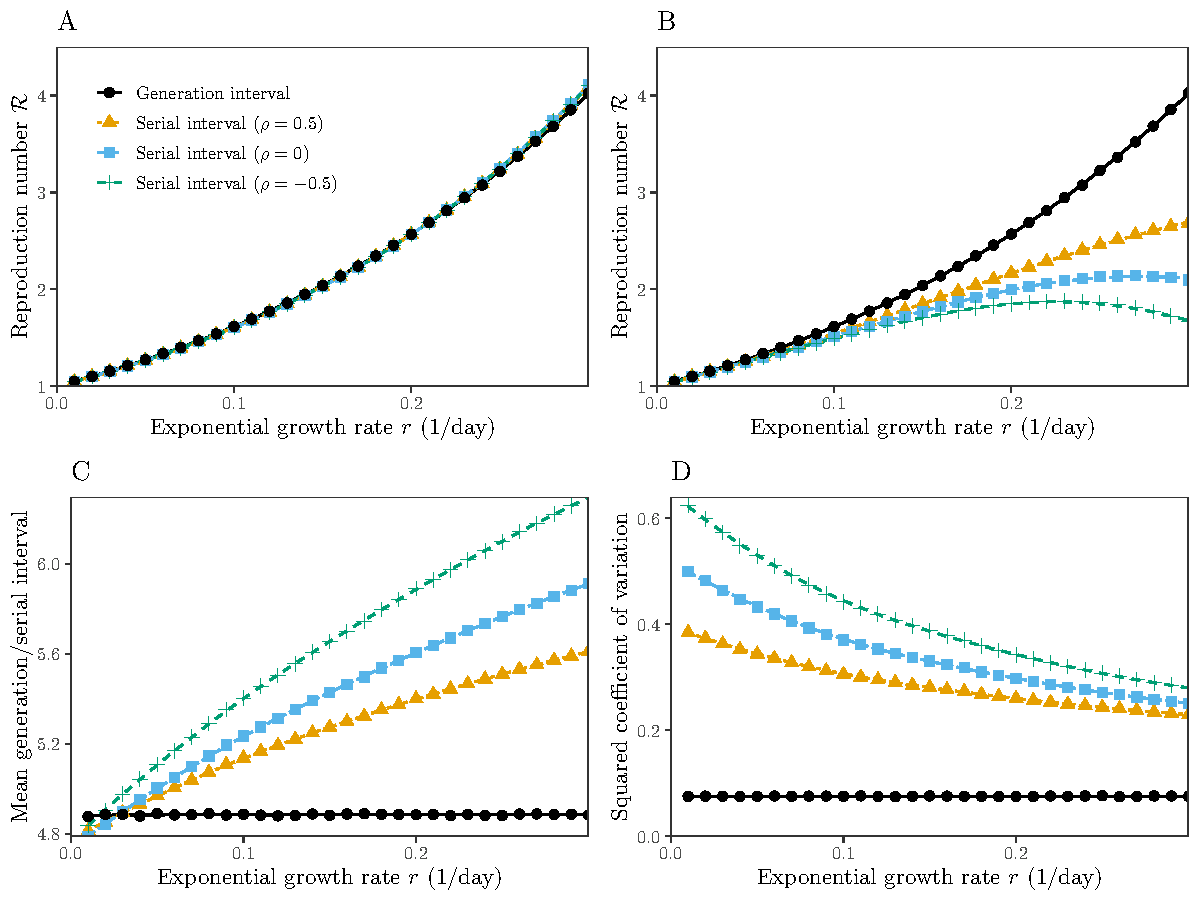
\includegraphics[width=\textwidth]{rR.pdf}
\caption{
\textbf{Estimates of the reproduction number from the exponential growth rate based on serial- and generation-interval distributions.}
(A). The forward serial-interval distribution during the exponential growth phase give a correct link between the exponential growth rate $r$ and the reproduction number \RR.
(B) The serial-interval distributions that assume that the backward incubation period of an infector and the forward incubation period of an infectee are identically distributed give an incorrect link between $r$ and \RR.
(C) The mean forward serial interval during the exponential growth phase depends on $r$.
(D) The squared coefficient of variation of forward serial intervals during the exponential growth phase depends on $r$.
}
\label{fig:rR}
\end{figure}

Comparing the shapes of initial forward serial-interval distributions and the intrinsic generation-interval distribution allows us to better understand how different distributions are able to give identical estimates of \RR.
In general, generation-interval distributions with higher means and less variability are expected to give higher \RR for a given $r$ \citep{wallinga2007generation, park2019practical}.
In this case, the initial forward serial intervals during the exponential growth phase have higher means (\fref{rR}C) and squared coefficients of variation (\fref{rR}D) than the intrinsic generation-interval distribution.
The effects of higher means (which increases \RR) and higher variability (which decreases \RR) cancel out exactly;
therefore, we can estimate the same \RR using both serial and generation intervals.

\begin{figure}[!ht]
\begin{center}
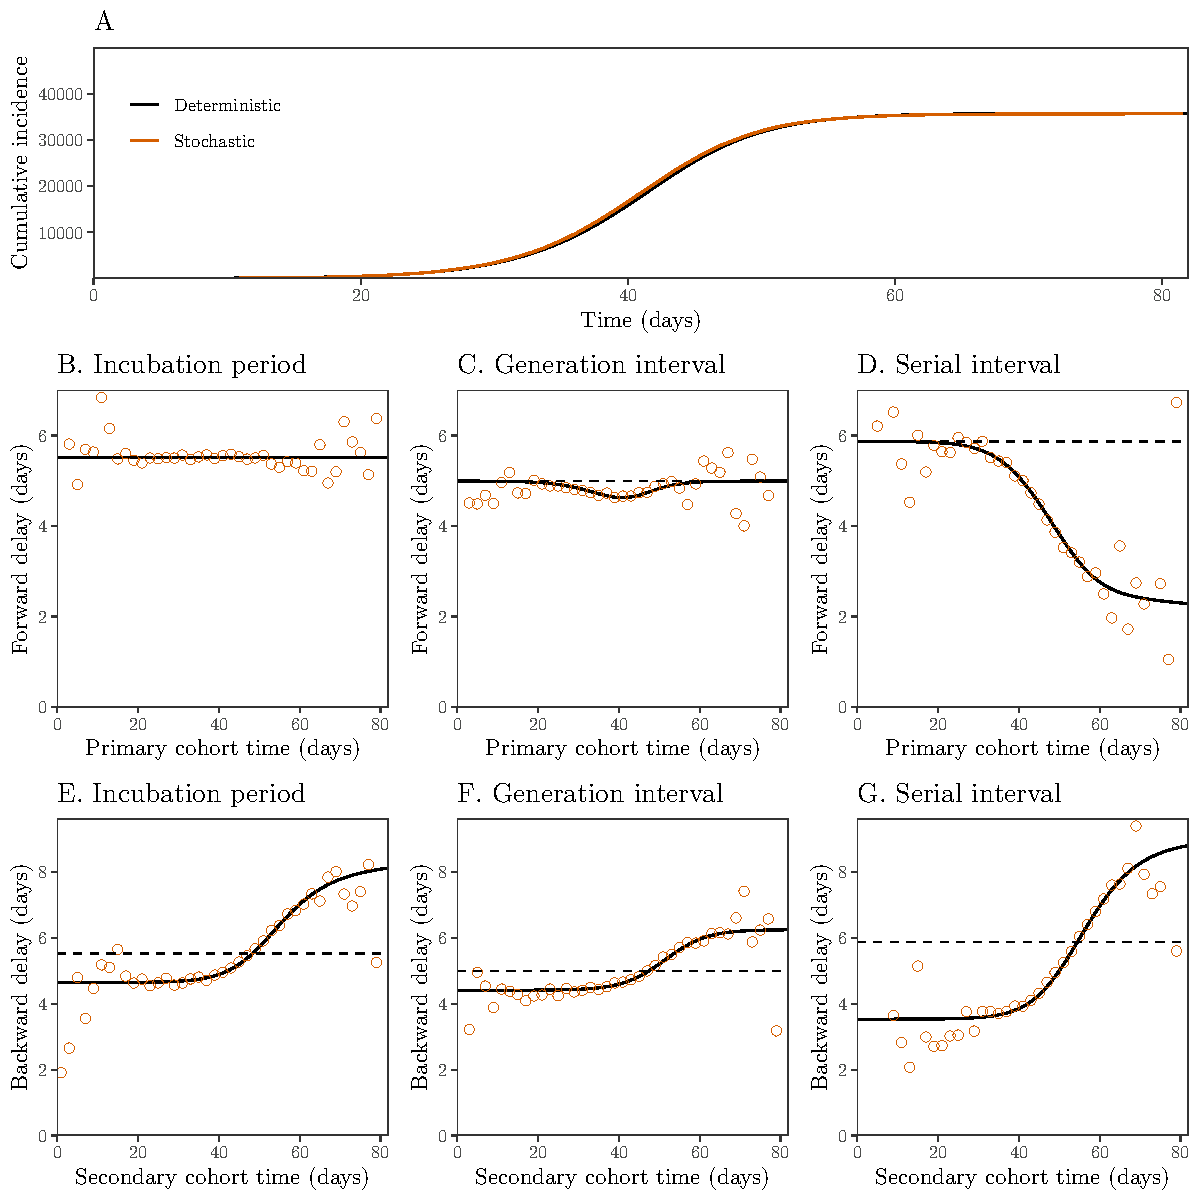
\includegraphics[width=0.95\textwidth]{forward.pdf}
\caption{
\textbf{Epidemiological dynamics and changes in mean forward and backward delay distributions.}
(A) Cumulative incidence over time.
(B--D) Changes in the mean forward incubation period, generation interval, and serial interval.
(E--G) Changes in the mean backward incubation period, generation interval, and serial interval.
Black lines represent the results of a deterministic simulation.
Orange lines and points represent the average of 10 stochastic simulations;
cumulative incidence from the stochastic simulations in panel A are shown without averaging.
Forward incubation periods and intrinsic generation-intervals are assumed to be independent of each other: $h(x_0, \sigma) = k(x_0) g(\sigma)$.
See Table 1 for parameter values.
}
\end{center}
\label{fig:epi}
\end{figure}

The initial forward serial interval distribution only applies to the exponential growth phase of an epidemic.
Now, we characterize how forward and backward serial intervals vary over the course of an epidemic when incubation periods and generation intervals are independent.
\fref{epi} compares the epidemiological dynamics (A) with the mean forward (B--D) and the mean backward (E--F) delay distributions of a deterministic model based on the renewal equation (\eref{renewal}) and of the corresponding stochastic realizations based on the Gillespie algorithm.
The mean forward incubation period remains constant throughout an epidemic as assumed (\fref{epi}B).
The mean forward generation interval decreases slightly as the epidemic progresses because an infected individual is less likely to infect another person as the proportion of susceptible individuals decreases (\fref{epi}C; \cite{kenah2008generation, champredon2015intrinsic}).
In contrast, the mean forward serial interval decreases over time (\fref{epi}D).

The forward serial interval distributions depend on three intervals (\fref{diagram}): (i) the backward incubation periods of infectors, (ii) the forward generation intervals, and (iii) the forward incubation periods of infectees.
Since both forward incubation period (\fref{epi}B) and generation-interval (\fref{epi}C) distributions remain roughly constant, changes in the forward serial-interval distributions are predominantly driven by changes in the backward incubation period distributions, whose mean increases over time (\fref{epi}D). 
In this case, the increase in the mean backward incubation period directly translates to the decrease in the mean forward serial interval.
We note that the relative contributions of the three distributions depend on their shapes and correlations between incubation periods and generation intervals --- as discussed earlier, the backward incubation period has \emph{no} effect on the forward serial intervals in the SEIR model, because transmission always occurs after symptom onset.

Qualitative patterns in the mean backward delays is robust across all delay distributions because they are predominantly driven by the changes in incidence (\fref{epi}D--F).
When incidence increases exponentially, individuals are more likely to have been infected more recently and therefore, we are more likely to observe shorter intervals.
When incidence decreases, we are more likely to observe longer intervals for similar but opposite reasons.
Since changes in incidence can occur even in the absence of significant susceptible depletion (e.g., due to intervention), we expect qualitative patterns in the changes of backward delay distributions to be robust across many outbreaks.

\begin{figure}[!ht]
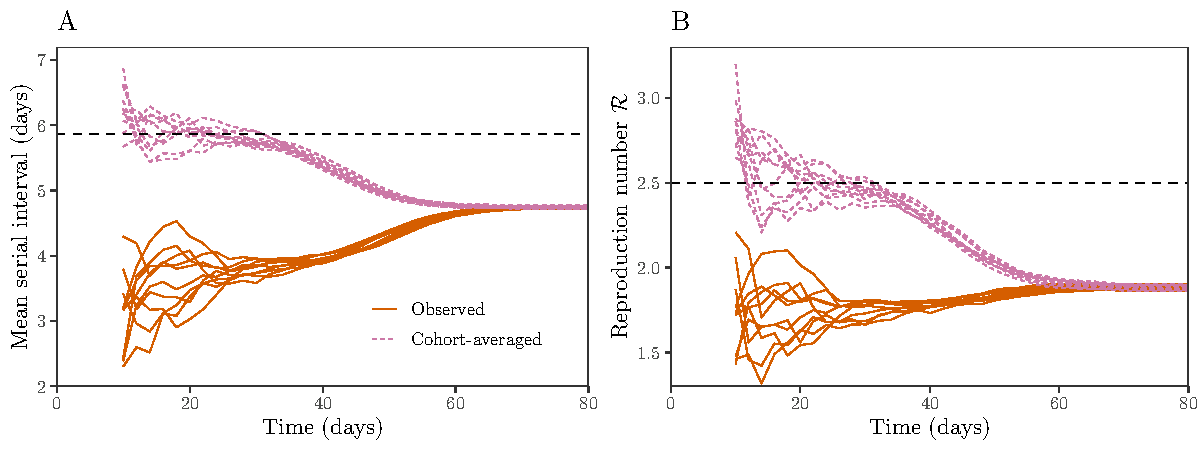
\includegraphics[width=\textwidth]{observedrR.pdf}
\caption{
\textbf{Estimates of the reproduction number from the observed serial intervals.}
(A) Changes in the observed and cohort-averaged mean serial interval over time.
(B) Changes in the estimate of \RR based on the observed and cohort-averaged mean serial interval over time.
Each line represents an independent stochastic realization.
}
\label{fig:obsrR}
\end{figure}

\subsection{Observed serial interval distributions}

Now, we turn to practical issues.
When an epidemic is ongoing, the observed serial intervals are subject to right-censoring because we cannot observe a serial interval if either an infector or an infectee has not yet developed symptoms.
\fref{obsrR} demonstrates how the effect of right-censoring in the observed serial intervals translates to the underestimation of \RR.
Notably, even if we can observe \emph{all} serial intervals across all transmission pairs after the epidemic has ended, we still underestimate the initial mean forward serial interval (\fref{obsrR}A) and therefore \Ro (\fref{obsrR}) by a large amount because the observed serial-interval distribution does not account for changes in the forward serial-interval distribution.
As the mean forward serial-interval distribution decreases over time, taking the average of all observed serial intervals throughout an epidemic will underestimate the mean of the initial forward serial-interval distribution, which provides the correct link between $r$ and \RR.

We provide a simple, heuristic way of assessing potential biases in the estimate of the mean initial forward serial interval and therefore \RR retrospectively.
Once serial intervals have been observed after the epidemic has been sufficiently progressed, we can group observed serial intervals by their primary cohort times (i.e., symptom onset times of infectors).
Then, we can compare how estimates of the mean serial interval as well as \RR change as we include more recent cohorts into the analysis (see `cohort-averaged' in \fref{obsrR}).
During the exponential growth phase, the estimates of the mean serial interval and \RR are consistent with the target value;
adding more data allows us to make more precise inference during this period.
However, the cohort-averaged estimates decreases rapidly soon after the exponential growth period.
This approach allows us to characterize potential biases in the estimates of \RR caused by changes in the forward serial-interval distributions.

\begin{figure}[!th]
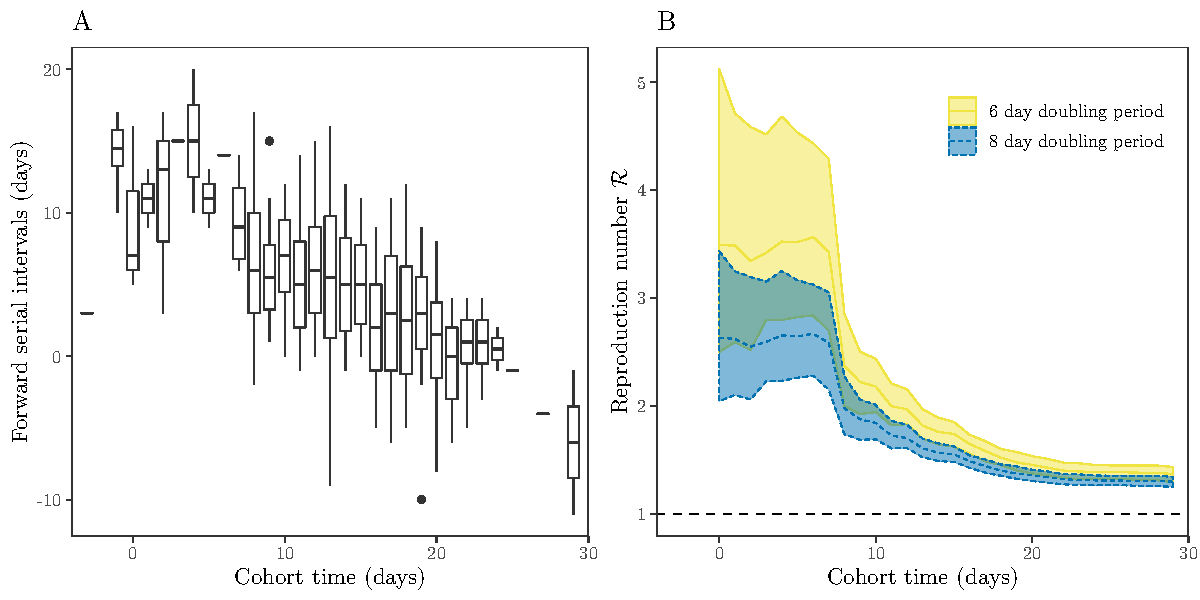
\includegraphics[width=\textwidth]{serial_analysis.pdf}
\caption{
\textbf{Observed serial intervals of COVID-19 and cohort-averaged estimates of \RR.}
(A--B) forward and backward serial intervals over time.
Points represent the means. Vertical error bars represent the observed maximum and minimum values.
Solid lines and ribbons represent the estimated locally estimated scatterplot smoothing (LOESS) fits and associated 95\% confidence intervals.
The dashed line represents the maximum observable delay for each primary cohort calculated from the most recent observed symptom onset date.
(C) Cohort-averaged estimates of \RR assuming doubling period of 6 and 8 days \citep{li2020early, wu2020nowcasting}.
Ribbons represent the associated 95\% bootstrap confidence intervals.
}
\label{fig:du}
\end{figure}

\subsection{Applications to the COVID-19 pandemic}

Finally, we reanalyze serial intervals of COVID-19 collected by \cite{du2020serial} from mainland China, outside Hubei province, based on transmission events reported between January 21--February 8, 2020;
\cite{du2020serial} estimated the mean serial of 3.96 days (95\% CI 3.53–4.39 days) and \Ro of 1.32 (95\% CI 1.16–1.48).
\fref{du}A shows that the mean forward serial interval decreases over time.
While the decrease is likely to be affected by the right-censoring (indicated by the closeness between the maximum observed serial intervals and maximum \emph{observable} serial intervals),  increase in the proportion of negative serial intervals are clearly indicative of the changes in the forward serial-interval distribution.
\fref{du}B shows that the mean backward serial interval increases over time.
While the qualitative changes in the mean forward and backward serial interval are consistent with our earlier simulations (\fref{epi}), the initial mean forward serial interval (\fref{du}A) appears to be larger than what we calculate earlier based on previously estimated incubation period and generation-interval distributions (\fref{rR}C).
These results indicate that previous estimates of incubation period and generation-intervals may have been underestimated as neither study explicitly accounts for right-censoring (Table 1).
%We do not explicitly account for the right-censoring as it is beyond the scope of this study.

\fref{du}C shows the cohort-averaged estimates of \Ro, which remain roughly constant until day 7 and suddenly decreases, as expected from our simulation study (\fref{obsrR}).
The estimates of \Ro based on the early forward serial intervals are also consistent with previous estimates of \Ro of the COVID-19 epidemic in China \citep{majumder2020early, park2020reconciling}.
We note that early cohort-averaged estimates of \Ro are unlikely to be affected by the right-censoring as we expect the degree of right-censoring to be low (\fref{du}A).
This example clearly demonstrates the danger of simply averaging the observed serial intervals and calculating the reproduction number using them.

\section{Discussion}

Characterizing generation- and serial-interval distributions is critical to understanding the outset of an outbreak as they determine the time scale of disease transmission.
Generation intervals measure the time difference between infection of a transmission pair, whereas serial intervals measure the time difference between symptom onset of a transmission pair \citep{svensson2007note}.
Due to their similar definitions, we show that their differences have been inaccurately captured previously.

Our study demonstrate the importance of defining a cohort for studying any epidemiological time delay distributions.
Previous studies have shown that generation interval can be either measured forward or backward \citep{champredon2015intrinsic};
we generalize their ideas and show that these ideas can be applied to all distributions.
Changes in the backward delay distributions is particularly robust across all distributions because they depend on previous changes in cohort sizes, which, in turn, depend on incidence of infection.
Previous analyses of COVID-19 epidemics have attempted to reconstruct the time series of symptomatic cases or infected cases from the reports of confirmed cases by assuming a constant backward delay distribution (e.g., \cite{tempvar, park2020potential, shim2020transmission}).
Although such approaches may be able to roughly match the time scale of an epidemic, we recommend using deconvolution approaches instead for proper reconstruction of epidemic time series \citep{goldstein2009reconstructing}.

Using cohort-based approaches, we define forward and backward serial intervals.
The forward serial-interval distribution describes the renewal process of the symptomatic individuals, and therefore, its initial distribution  provides the correct link between $r$ and \RR.
While our results support the use of serial interval distributions for calculating \RR, 
they also reveal gaps in current approaches to characterizing serial intervals.
Previous studies have (i) recommended using up-to-date serial intervals \citep{thompson2019improved}, (ii) assumed that the serial interval distribution remains constant throughout an epidemic \citep{wallinga2004different, cori2013new}, and (iii) applied serial interval distributions estimated from one location to analyzing epidemics in other locations \citep{tempvar};
however, all of these approaches implicitly ignore spatiotemporal variation in incidence, which affects the serial-interval distributions, and may therefore give systematically biased estimates of \RR. 
For example, given large geographical differences in the observed exponential growth rates of the COVID-19 epidemic \citep{tempvar}, the initial forward serial interval distributions is likely to vary across different countries.
Future studies should aim to characterize spatiotemporal variation in serial intervals and understand the drivers of their differences.

We also show that there are multiple serial-interval distributions that correspond to the same set of generation-interval and incubation period distributions depending on their correlations.
Conversely, this means that not explicitly accounting for their correlations can bias the estimate of the intrinsic generation-interval distribution from the serial-interval distribution.
Furthermore, previous studies that tried to estimate the generation-interval distributions from the observed serial intervals often ignored the differences between the backward incubation period of an infector and the forward incubation period of an infectee (e.g., \cite{klinkenberg2011correlation, ganyani2020estimating}).
There is currently a need for better statistical tools for teasing apart the intrinsic generation-interval distributions from the observed serial intervals.

Our study is not without limitations.
Here, we assumed that all individuals develop symptoms and that the the entire transmission process (e.g., direction of transmission, symptom onset dates, infection dates, etc.) are observable.
In practice, asymptomatic and presymptomatic transmission of COVID-19 makes measuring serial intervals difficult \citep{bai2020presumed,he2020temporal,wei2020presymptomatic}.
For example, symptom onset dates cannot be used as a reliable proxy for the direction of transmission as infectees may develop symptoms before their infectors.
Based on the COVID-19 parameters (Table 1), we expect roughly 3\% of infectees to develop symptoms before their infectors during the exponential growth period; 
this probability increases as epidemic progresses because backward incubation period of an infector increases.
Biases in the observed serial intervals will necessarily bias the estimates of \RR. 
Furthermore, serial intervals do not take into account asymptomatic transmission; 
not explicitly accounting for asymptomatic transmission may also bias the estimates of \RR \citep{park2020time}.

Despite these limitations, our analysis of serial intervals of COVID-19 provide further support for our theoretical framework, demonstrating temporal variation in serial intervals and their effects on the estimates of \RR.
To our knowledge, most, if not all, existing estimates of the serial-intervals of COVID-19 implicitly or explicitly assume that the serial-interval distributions remain constant throughout the course of an epidemic \citep{du2020serial, he2020temporal, nishiura2020serial,tindale2020transmission,zhao2020estimating,zhang2020evolving}.
Our study provides a rationale for reassessing estimates of serial-interval distributions of the COVID-19 pandemic.

\pagebreak

\section{Appendix}

\subsection{Deterministic simulation}

We simulate the renewal equation model using a discrete-time approximation:
\begin{equation}
\begin{aligned}
i(t) &= \Ro S(t-\Delta t) \sum_{m=1}^{\ell} i(t-m \Delta t) \hat{g}(m \Delta t) \\
S(t) &= S(t-\Delta t) - i(t)
\end{aligned}
\end{equation}
where $\hat{g}$ is a discrete-time intrinsic generation-interval distribution that satisfies the following:
\begin{equation}
\hat{g}(m \Delta t) = \frac{g(m \Delta t)}{\sum_{i=1}^\ell g(m \Delta t)}, \quad m=1, \dots, \ell
\end{equation}
The continuous-time intrinsic generation-interval distribution is parameterized using a log-normal distribution (Table 1). We define the forward incubation period distribution in a similar manner:
\begin{equation}
\hat{k}(m \Delta t) = \frac{k(m \Delta t)}{\sum_{i=1}^\ell k(m \Delta t)}, \quad m=1, \dots, \ell,
\end{equation}
where its continuous-time analog is also based on a log-normal distribution.
For brevity, we assume that the forward incubation periods and intrinsic generation intervals are independent:
\begin{equation}
\hat{h}(m \Delta t, \Delta t n) = \hat{k}(m \Delta t)\hat{g}(\Delta t n), \quad m,n=1, \dots, \ell.
\end{equation}
We use $\Delta t = 0.025\,\textrm{days}$ and $\ell=2001$ for discretization steps.

We initialize the simulation with population size $N$=40,000 as follows:
\begin{equation}
\begin{aligned}
i(m \Delta t) &= C \exp(r m \Delta t), \quad m=1, \dots, \ell\\
S(m \Delta t) &= N - \sum_{n=1}^m i(m \Delta t), \quad m=1, \dots, \ell\\
\end{aligned}
\end{equation}
where $C$ is chosen such that $\sum_{n=1}^\ell i(m \Delta t)=10$.
These initial conditions allow the model to follow exponentially growth from time $\Delta t (\ell + 1)$ without any transient behaviors.
Results presented in the main text show simulations beginning from time $\Delta t (\ell + 1)$.

\subsection{Stochastic simulation}

We run stochastic simulations of the renewal equation model using an individual-based model on a fully connected network (i.e., homogeneous population) based on the Gillespie algorithm that we developed earlier \citep{park2019inferring}.
First, we initialize an epidemic with $I(0)$ infected individuals (nodes) in a fully connected network of size $N$. 
For each initially infected individual, we draw number of infectious contacts from a Poisson distribution with the mean of \Ro and the corresponding generation intervals for each contact from a log-normal distribution (Table 1).
Contactees are uniformly sampled from the total population.
All contactees are sorted into event queues based on their infection time.
We update the current time to the infection time of the first person in the queue.
Then, the first person in the queue makes contacts based on the Poisson offspring distribution described earlier and their contactees are added to the sorted queue.
Whenever contactees are added to the sorted queue, we remove all duplicated contacts (but keep the first one) as well as contacts made to individuals that have already been infected.
Simulations continue until there are no more individuals in the queue.
We simulate 10 epidemics with $I(0)=10$ and $N$=40,000.

\subsection{Linking $r$ and \RR using serial-interval distributions}

The intrinsic generation-interval distribution $g(\tau)$ provides a link between $r$ and \RR via the Euler-Lotka equation:
\begin{equation}
\frac{1}{\RR} = \int_0^\infty \exp(-r\tau) g(\tau) \mathrm{d} \tau.
\end{equation}
Here, we prove that the initial forward serial-interval distribution $f_0$ also provides the same link:
\begin{equation}
\frac{1}{\RR} = \int_{-\infty}^\infty \exp(-r\tau) f_{0}(\tau) \mathrm{d} \tau,
\end{equation}
where the initial forward serial-interval distribution is defined as:
\begin{equation}
f_{0}(\tau) \propto \int_{0}^{\infty} \int_{0}^{\max(0,x+\tau)} \exp(-rx) h(x, \sigma) k(x-\sigma+\tau) \mathrm{d}\sigma\,\mathrm{d}x.
\end{equation}

First, we rewrite the initial forward serial-interval distribution in the following form:
\begin{equation}
\begin{aligned}
f_{0}(\tau) &\propto \int_0^\infty \int_{-\alpha_1}^{\tau} \exp(-r\alpha_1) h(\alpha_1, \alpha_2 + \alpha_1) k(\tau - \alpha_2) \mathrm{d}\alpha_2\,\mathrm{d}\alpha_1\\
&= \int_{-\infty}^{\tau} \int_{\max{(0,-\alpha_2)}}^{\infty} \exp(-r\alpha_1) h(\alpha_1, \alpha_2 + \alpha_1)k(\tau - \alpha_2)\mathrm{d}\alpha_1\, \mathrm{d}\alpha_2\\
\end{aligned}
\end{equation}
It follows that $z(\alpha_2)$ describes the time between symptom onset of infector and infection of infectee:
\begin{equation}
z(\alpha_2) \propto \int_{\max{(0,-\alpha_2)}}^{\infty} \exp(-r\alpha_1) h(\alpha_1, \alpha_2 + \alpha_1) \mathrm{d}\alpha_1.
\end{equation}
The initial forward serial-interval distribution $f_0$ can be expressed as a convolution of $z$ and $k$:
\begin{equation}
\begin{aligned}
f_{0}(\tau) &\propto \int_{-\infty}^{\tau} z(\alpha_2) k(\tau - \alpha_2) \mathrm{d}\alpha_2.\\
\end{aligned}
\end{equation}
Then, we have
\begin{equation}
\int_{-\infty}^\infty \exp(-r\tau) f_{0}(\tau) \mathrm{d} \tau = \int_{-\infty}^\infty \exp(-r\tau) z(\tau) \mathrm{d} \tau \int_{0}^\infty \exp(-r\tau) k(\tau) \mathrm{d} \tau
\end{equation}

Note that 
\begin{equation}
\begin{aligned}
&\int_{-\infty}^\infty \int_{\max{(0,-\alpha_2)}}^{\infty} \exp(-r\alpha_1) h(\alpha_1, \alpha_2 + \alpha_1) \mathrm{d}\alpha_1 \mathrm{d}\alpha_2\\
&= \int_{0}^\infty \int_{-\alpha_1}^\infty \exp(- r \alpha_1) h(\alpha_1, \alpha_2+\alpha_1) \mathrm{d}\alpha_2\,\mathrm{d} \alpha_1\\
&= \int_{0}^\infty \exp(- r \alpha_1) k(\alpha_1) d\alpha_1
\end{aligned}
\end{equation}
because $k$ is a marginal probability distribution of $h$.
Since $\int_{0}^\infty \exp(- r \alpha_1) k(\alpha_1) d\alpha_1$ is a normalization factor for probability distribution $z$, we have:
\begin{equation}
\int_{-\infty}^\infty \exp(-r\tau) z(\tau) \mathrm{d} \tau = \frac{\int_{-\infty}^\infty \exp(-r\tau) \int_{\max{(0,-\alpha_2)}}^{\infty} \exp(-r\alpha_1) h(\alpha_1, \alpha_2 + \alpha_1) \mathrm{d}\alpha_1 \mathrm{d}\tau}{\int_{0}^\infty \exp(- r \alpha_1) k(\alpha_1) d\alpha_1}.
\end{equation}
Then, we have:
\begin{equation}
\int_{-\infty}^\infty \exp(-r\tau) f_{0}(\tau) \mathrm{d} \tau = \int_{-\infty}^\infty \exp(-r\tau) \int_{\max{(0,-\alpha_2)}}^{\infty} \exp(-r\alpha_1) h(\alpha_1, \alpha_2 + \alpha_1) \mathrm{d}\alpha_1 \mathrm{d}\tau.
\end{equation}

We are left to show that 
\begin{equation}
\int_0^{\infty} \exp(-r\tau) g(\tau) \mathrm{d}\tau = \int_{-\infty}^\infty \exp(-r\tau) \int_{\max{(0,-\alpha_2)}}^{\infty} \exp(-r\alpha_1) h(\alpha_1, \alpha_2 + \alpha_1) \mathrm{d}\alpha_1 \mathrm{d}\tau,
\end{equation}
where the intrinsic generation-interval distribution $g$ is also a marginal probability distribution of $f$:
\begin{equation}
g(\tau) = \int_0^\infty h(\alpha_1, \tau)  \mathrm{d} \alpha_1.
\end{equation}
Let $\sigma = \alpha_1 + \tau$. Then, by change of variables, it immediately follows that
\begin{equation}
\begin{aligned}
&\int_{-\infty}^{\infty} \exp(-r\tau) \int_{\max(0, -\tau)}^\infty \exp(- r \alpha_1) h(\alpha_1, \tau+\alpha_1) \mathrm{d} \alpha_1\, \mathrm{d}\tau\\
&=\int_{0}^{\infty} \int_{0}^\infty \exp(- r \sigma) h(\alpha_1, \sigma) \mathrm{d} \alpha_1\, \mathrm{d}\sigma\\
&=\int_{0}^{\infty} \exp(-r\tau) g(\tau) \mathrm{d}\tau
\end{aligned}
\end{equation}
Therefore, the initial forward serial--interval distribution and the intrinsic generation-interval distribution give the same link between $r$ and \RR.

\bibliography{serial}

\end{document}
